\documentclass[12pt]{report}
\usepackage{nopageno}
\usepackage{xcolor} % for different colour comments
\usepackage{parskip} % Space between each paragraph.
%\usepackage{hardwrap} % for text length of 80 pts
\usepackage[margin=1.2in]{geometry}
\usepackage{hyperref}
\usepackage{../ltx/edcomms}
\usepackage{graphicx}
\usepackage[section]{placeins} % Prevents floats from floating across sections
\usepackage{natbib}%Bibtex

\usepackage{ifthen}
\usepackage{../ltx/edcomms}

%% Comments are enabled and disabled by 'draft' mode. I hacked in my own draft
%% mode (https://en.wikibooks.org/wiki/LaTeX/Macros) because the LaTeX draft
%% mode disables a bunch of things that I don't want it to. I just want it to
%% disable comments. Do not set any of this manually, just use the build script,
%% which builds both draft and final copies. Comments are enabled by default, so
%% if you build manually, you get a draft copy. 
\providecommand\draftmode{true}

\ifthenelse{\equal{\draftmode}{true}}{
\newcommand{\authornote}[3]{\textcolor{#1}{[#3 ---#2]}}
\newcommand{\todo}[1]{\textcolor{red}{[TODO: #1]}}
%\edcommstrue %% Dr. Kahl's comment package. Eventually we should migrate all
             %% comments to this.
}{
\edcommsfalse 
\newcommand{\authornote}[3]{}
\newcommand{\todo}[1]{}
}

% wss = Dr. Smith ; ds = Dr. Szymczak
\newcommand{\wss}[1]{\authornote{magenta}{SS}{#1}}
\newcommand{\ds}[1]{\authornote{blue}{DS}{#1}}



\setlength{\parindent}{15pt} % parskip sets this to 0. 15 is default.

%%%%%%%%%%%%%%%	START OF DOCUMENT %%%%%%%%%%%%%%%%%%%%
\edcommsfalse
\begin{document}

\begin{titlepage}\begin{center}

\vspace*{1cm}

{\Huge\textbf{Ampersand Event-Condition-Action Rules}}

\vspace{0.5cm}
{\Large Software Requirement Specification 
	
	\edinsert{JG}{Version 1}

\vspace{1.5cm}
Yuriy Toporovskyy,\ Yash Sapra,\ Jaeden Guo}
\vfill

We acknowledge that this document uses material from the Volere Requirements
Specification Template, copyright 1995 - 2012 the Atlantic Systems Guild
Limited.

\vspace{0.8cm}
\end{center}
CS 4ZP6 \\
October 9th, 2015 \\ 
Fall 2015 / Winter 2016 
\end{titlepage}

%% Revision history
\begin{table}[ht!]\begin{center}
\caption{Revision History}  
\begin{tabular}{|l|l|l|}\hline
\textbf{Author} & \textbf{Date} & \textbf{Comment} \\\hline 
Yuriy Toporovskyy & 26 / 09 / 2015 & Initial skeleton version \\\hline
\end{tabular}
\end{center}\end{table}

\tableofcontents
\listoffigures
\listoftables

%% \clearpage

%%%%%%%%%%%%%%%%%%%%%%%%%%%%%%%%%%%%
%% Chapter 1: ???                 %%
%%%%%%%%%%%%%%%%%%%%%%%%%%%%%%%%%%%%
\edchange{JG}
{\chapter{Introduction}\label{ch:Intro}}
{\chapter{Project Drivers}\label{ch:Drivers}}

\edchange{JG}
{\section{Project Description}\label{sec:Intro}}
{\section{The Purpose of the Project}\label{sec:Purpose}}
\edcomm{JG}{any comments I made, is a suggestion and its up to you which way 
you prefer to write it. thanks for getting this to us early, I'm sorry we're so 
unorganized}
%% 1a. The User Business or Background of the Project Effort
A large part of designing software systems is requirements engineering. One
of the greatest challenges of requirements engineering is translating from
business requirements to a functional specification. Business requirements are
informal, with the intention of being easily understood by humans; however,
functional specifications are written in formal language to unambiguously capture attributes of the 
information system. Typically, this translation
of business requirements to a formal specification is done by a requirements
engineer, which can be prone to human error.

Ampersand is a tool which aims to address this problem in a different way; by
translating business requirements written in natural language into a formal
specification by means of a ``compilation process'' (\cite{derFun}). 
\edcomm{JG}{Maybe we should cut out how entirely, because there's a design 
specification -- and solely focus on what? thoughts?}%
\edcomm{YT}{The significance of Ampersand has to do with how it solves the
  problem, or how it works. To speak to the purpose of the project means to
  explain why the Ampersand solution is good and why we are spending our time
  making it better. The rubric has a section titled 'General System
  Description', so we need to say something about it}%
%% NB: Put a tex comment at
%% the end of the line after your 'in-line' comments, or latex inserts extra
%% whitespace when rendering with comments off.
Even though the business requirements and formal specification are written in
entirely different languages, the ``compiler guarantees compliance between the
two'' (\cite[p.~2]{derFun}). 

Ampersand also provides engineers with a variety of aids which
help them to design products that fulfill all of the needs of their clients and
the end-users (Figure~\ref{fig:figure1}); including data models, service catalogs and their
specifications. Requirements engineering is perhaps most important in
safety-critical systems; to this end, Ampersand generates modeling aids and
specifications which are provably correct (\cite{derFun}). 

\begin{figure}
  \centering
    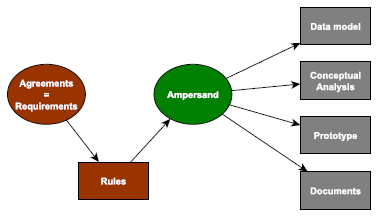
\includegraphics[width=0.7\textwidth]{../figures/ampersand_artifacts}
\caption{Ampersand produces a set of artifacts based on user's requirements.}~\label{fig:figure1}
\end{figure}

%% 1b. Goals of the Project 
Ampersand has proven reliable in practical situations, and there have been
efforts to teach this approach to business analysts. A large portion of the
Ampersand system is already in place; the primary focus of this project is to
augment Ampersand with increased capabilities for automation.

For example, consider a system for ordering products online. Ampersand takes, as
an input, statements of business requirements like
\edcomm{JG}{Good example, could we put something in here about restrictions of 
of the real world?}%
\edcomm{YT}{Business requirements *are* real world requirements. Do you mean something safety-related?
This example isn't the best, I know, but I deliberately chose a simple example}%
\edcomm{YS}{The example is easy to understand. I think we should keep it.} 
\edcomm{YS}{I'm not too sure if the haskell implementation needs to be a part of the introduction.
Rubrics indicate the following critera - - - - %%%%%%%%%%%%%%%%%
 delineate purpose, specify intended audience), system scope, definitions, acronyms,
abbreviations, references, system overview, roadmap of report - - - -
%%%%%%%%%%%%%%%%%%%%%%%
I believe we miss definition of E.F.A and E.C.A since it is being used a lot in the document
}%
\edcomm{YT}{Haskell isn't mentioned at all the intro, ECA is mentioned but is also defined
(it is really quite simple, we don't define it mathematically, just in natural language, so 
it shouldn't be incomprehensible).}%
\begin{quotation}
\noindent{\emph{Every order must have a customer and a list of products; and the total price on
the order must equal the sum of the prices of the products.}}
\end{quotation}
\edcomm{YS}{Attempt at defining ECA}%
\edcomm{YS}{Should we remove some of the haskell code and define the scope of our project in terms of conserving these data rules instead? There's a good chance Dan hasn't read our new problem statement so he doesn't necessarily have a clear idea of Ampersand. Suggestions?}\edcomm{YT}{There is no Haskell code!}\edcomm{YS}{Sorry, i meant the pre-post conditions pairs, I guess we'll let that stay.}%
These are translated into, among other things, formal rules concerning how the
information system must react to changes in its state. Ampersand describes these rules as
a set of Event-Condition-Action Rules (referred to as the E.C.A rules hereafter)
that specify when an event takes place under a given condition, what Action the software must take. 
The information system may contain a function for manipulating orders. (Ampersand can also generate
prototype software models, including functions types like these, from business
requirements - but this is not the topic of our contribution). For example,

\begin{verbatim}
addToOrder : ( o : Ref Order, t : Product )
\end{verbatim}
\noindent{where \verb|Ref x| represents the type of references to values of type
\verb|x|; \verb|Order| and \verb|Product| the types of orders and products, respectively.  }

Ampersand can generate pre- and post-conditions for this function, based on the
business requirements. This constitutes a formal specification of the
information system. For example, the above function may have the following specification:

\begin{verbatim}
{ PRE: o.totalCost = t0 } 
addToOrder(o,t) = ...
{ POST: o.totalCost = t0 + t.cost } 
\end{verbatim}

It is proven \edcomm{YT}{This is 'proven' because someone told me we have a
  proof/presentation of the algorithm, but not its implementation. Can anyone
  find this? We absolutely need a reference to this.} \edcomm{JG}{Can you give 
  me more context as to what is proven? I found an article on ampersand 
  subsets, I pushed it; look for "subsets" by Joosten(both)}%
\edcomm{YT}{There is no file in the repository with the word 'subset' in it?}%
that for the subset of processes which Ampersand can support, there is an
algorithm which will generate the necessary code to satisfy the post-conditions
(ie, formal specifications) of each function. However, Ampersand does not yet
implement this algorithm. Currently, a user of Ampersand must manually indicate
how each violation must be corrected.

In the previous example, the implementation of the
function could be as follows: 

\begin{verbatim}
{ PRE: o.totalCost = t0 } 
addToOrder(o,t) = 
  o.orders.append(t);
  o.totalCost = o.totalCost + t.cost;
{ POST: o.totalCost = t0 + t.cost } 
\end{verbatim}

The first line includes the item in the order, and the second line fixes the
violation of the post-condition which would occur without it. Currently this
second line would have to be hand-written by the programmer, but the
afformentioned \edcomm{YT}{Should have a name to refer to the algorithm
  somehow?} algorithm can derive it from the business rules. The main
contribution of this project will be to implement the algorithm which generates
the code to fix violations.

\section{The Stakeholders}\label{sec:Stakeholders}
%% From the template:
%% For each type of stakeholder, provide the following information:
%% ● Stakeholder identification (some combination of role/job title, person name, and organization name)
%% ● Knowledge that the project needs from that stakeholder
%% ● The degree of involvement necessary for that stakeholder/knowledge combination
%% ● The degree of influence for that stakeholder/knowledge combination
%% ● Agreement on how to address conflicts between stakeholders who have an interest in the same knowledge
%% This doesn't really seem to fit a list format.. And the majority of these things apply
%% mainly to Ampersand - everyone else only uses Ampersand, the developers of Ampersand
%% themselves also need our code to fit into their project, so they have the majority of the say
%% in how things are done. Namely:
%%    A list of the decisions for which the client will be responsible
%% Most 'decisions' will be made by them. 
%% TODO: Write this section. 

\edcomm{YT}{These are the only real stakeholders I can think of...}
\subsection{Ampersand Designers}\label{subsec:Ampersand}
Ampersand designers include Dr. Stef Joosten, Dr. Sebastian Joosten and Dr. 
Wolfram Kahl, who in addition to supervising the development of E.F.A are also 
Ampersand contributers. Dr. Stef Joosten is the designer of the Ampersand 
method which have been successfully implemented in various public sectors. The 
interest stemming from these three individuals are not only professional but 
also personal. Ampersand has been nurtured by a great deal of patience and 
dedication. The designers of E.F.A by extension are Ampersand contributors and 
are affected by its outcome, the piece of Ampersand we will build is a 
necessary component required for completion of undergraduate and is designed to 
test the capabilities of an undergraduate team. 
These individuals are the foundation of the belief system by which Ampersand is 
built. The Ampersand model is built on the belief that technology is highly 
incorporated in the use of business and affects the life of every individual. 
It is the belief that information system can and will be designed and built at 
an affordable price and perfectly compliant with the functionalities that users 
desire. This perspective treats information systems as a commodity of the real 
world that can be traded, altered, and used by any individual who is willing to 
learn how to use it.
\subsection{Requirements engineers}\label{subsec:BusReq}
Requirement engineers are responsible of translating business 
requirements into project specifications. Ampersand provides requirement 
engineers with the freedom to explore their creativity rather than be tried 
down by technical minutes. The ability to delegate time consuming tasks such as 
manually checking over technical specifications would increase the efficiency 
of the task at hand as well as decrease the number of hours required for 
completion. An added benefit which engineers receive is the ability to confirm 
that the system they have designed matching the specifications given to them by 
the client. E.F.A provides the ability to ensure no contradictions are found 
within the design by automatically fixing inconsistency that may arise. 
\subsection{Architects \& Functional Specification Designers}
System architects, similar to functional specification designers are 
responsible for various designs which affect procedure and processes in a place 
of business. Ampersand has the ability to confirm that the design provided by 
the Architect matches any building regulations that must be meet. Regardless of 
whether the specification is for safety or aesthetics, the product must meet the 
client's requirements and minimal legal regulations. Ampersand is able to 
compose rules and regulations for data which fully incorporates both without 
contradiction. The addition of E.F.A allows Ampersand to automate correction  
on data which may contradict rules specified for a project. Architects and 
functional specification designers will be able to take advantage of the 
numerous resources Ampersand can provide such as automatic generation of 
databases within prototypes along with tables and relational schema's. 
Furthermore, there is a full range of graphics that stakeholders can choose 
from in order to provide visual display of their design which user may find 
more friendly and easy to understand. 
\subsection{Process Innovators}
Process innovators covers a broad range of individuals that would not commonly 
be considered stakeholders. This broad category includes anyone who provides 
input for business processes which includes both sides of a business agreement, 
in addition to individuals who play a role in seeing the completion of a 
business process. Ampersand allows continuous input as a living system and has 
the ability to reorganize requirements when new constraints are added, and 
E.F.A has the ability to assure the correctness of system information relative 
to the requirements it has been given. With E.F.A's ability to verify 
inconsistencies and automate their correction, changes to design and 
restrictions due to unforeseen circumstances can be added without a system 
overhaul. The efficiency in which Ampersand can provide has the potential to 
dramatically decrease flaws that commonly litter information system.

\subsection{Software engineers}\label{subsec:SftwReq}

%%%%%%%%%%%%%%%%%%%%%%%%%%%%%%%%%%%%
%% Chapter 2: Project Constraints %%
%%%%%%%%%%%%%%%%%%%%%%%%%%%%%%%%%%%%
\chapter{Project Constraints}\label{ch:Constraints}
The main constraint of this project is time; this is limited to the 8 month 
period in which we have to build it. It is difficult to perfect an internal 
construction without a large system in such a short amount of time. But time 
restraint is an obstacle which all projects face, because it is not limitless. 
Another major constraint that most project face that this project does not 
require is the financial constraint where projects become difficult to maintain 
and often halt in their progress due to monetary constraints. The lack of 
monetary constraints due to the open source software opens up a broad base of 
opportunities for future improvements and limitless contributions from the 
community.
\section{Mandated Constraints}\label{sec:Constraints}

%%%%
%% 4.1 Solution constraints. 
%% We don't have that many, so 'solution constraints' isn't really appropriate.
\subsection{Project philosophy}

Ampersand is an existing software project with a very sizable code base. The
cost of maintaining poorly-written code can be very high and can outweigh the
benefit of the contribution. In order for our code to eventually be merged into
Ampersand, it must be maintainable: it must be written according to coding
practices of Ampersand; it must be well documented, so it can be easily
understood by other programmers. 

Similarly, our code must not introduce any errors or performance regressions
into Ampersand. Our code must satisfy existing tests and additional tests should
be written for the new algorithm being implemented. Writing maintainable and
well-documented code will help with this goal as well.

These motivations are very important to Ampersand and are considered primary
goals alongside the obvious goal of producing code implementing the desired
feature.

%%3b.
\subsection{Implementation environment}
\subsubsection*{Haskell}
The Ampersand code base is written almost entirely in Haskell. Part of the
prototype software is written in PHP and Javascript %Ref???  
but we likely do not have to interact with this code base. Our code contribution
must be entirely in Haskell.

\subsubsection*{Haskell software}
Ampersand is designed to be used with the Glasgow Haskell Compiler (from here on, GHC) %%REF
and the associated cabal build system. %%Ref
Ampersand also uses many open source Haskell packages, all available on the
Hackage package archive. %% Ref. 
We may not use additional packages. %% Or can we? Maybe if we really needed
                                    %% something, we could ask. But probably not...


\subsubsection*{GitHub}
The Ampersand code base currently lives on GitHub. Our code contributions must
also be on GitHub; this will facilitate easy integration of our code into
Ampersand. This is especially useful if only parts of our code eventually become
integrated into Ampersand - GitHub facilitates this especially. 
\edcomm{YS}{Do we want to tell them that our code might not be integrated in Ampersand?
I think we should abstract this information to make our configuration look more significant.}%

\subsubsection*{Graphviz}
Graphiv is open source graph visualization software, which has the ability to
visually represent information in the form of charts and graphs. It contains
various designs from which the user is able to select. This is used to take
descriptions of graphs in simple text and create diagrams. Ampersand generates
reports about the input system using graphs and charts, so this is one of the
basic components required to run Ampersand.

\subsubsection*{XAMPP}
Ampersand generates prototype websites based on business requirements; to run
these, some web server software is needed. XAMPP stands for cross \big( i.e., X
\big) platform Apache distribution containing MySQL, PHP and Perl. XAMPP \cite{xampp} is the
most convenient way to set up a working database for Ampersand and access .php
pages. 

\edcomm{YT}{Be liberal with what you include in this section, but if it is a
  'technology' then put it in the previous section. Any acronyms, or words that
  the layman probably won't know, need to be here.}%
\section{Naming Conventions and Terminology}\label{sec:Naming} 
\begin{description}
\item[ECA] Stands for Event-Condition Action. The rule structure used for data
  bases and commonly used in market ready business rule engines. ECA rules are
  used in Ampersand to describe how a database should be modified in response to
  a system constraint becoming untrue. Event-Condition Action rules have
  the following structure:
%TODO: cite rule 
%design.p:8-9
\begin{verbatim}
when <some event has happened> 
and if <some condition is fulfilled> 
    do <this activity>
\end{verbatim} %TODO{JG}: bold or italicize words in definitions
\item [EFA] Stands for ``ECA (see above) for Ampersand''.
\item [Functional specification] A \emph{formal} document which details the operation,
  capabilities, and appearance of a software system. 
\item [Requirements engineering] The process of translating business
  requirements into a functional specification. 
\item [Business requirements] Requirements which exist due to some real world constraints;
  ie, financial, logistic, physical or safety constraints. 
\item [Business rules] See \emph{Business Requirements}.
\item [Natural language] Language written in a manner similair to that of human communication; 
  language intended to be interpreted and understood by humans, as opposed to machines. 
\item [ADL] Stand for ``Ampersand Definition Language''. From a given set of
formally defined business requirements, ADL generates a functional specification
consisting of a data model, a service catalog, a formal specification of the services,
and a function point analysis. An ADL script acts as an input for Ampersand.
\edcomm{YS}{ADL is probably not "A data Language".}
\edcomm{YT}{I swear to god I read "A data Language" somewhere... maybe I was
  delirious from lack of sleep... In any case, we should eventually find a
  reference for ``ADL'', whatever it is...}
\end{description}
%TODO{JG}: add Expression as a data type? Find a better way of describing 
%Expression without implementation details

%% This section is strange and we may have to replace it with something else...
\section{Relevant Facts and Assumptions}\label{sec:Assumptions}

%%%%%%%%%%%%%%%%%%%%%%%%%%%%%%%%%%%%%%%%%%
%% Chapter 3 -- Functional requirements %%
%%%%%%%%%%%%%%%%%%%%%%%%%%%%%%%%%%%%%%%%%%
\chapter{Functional Requirements}\label{ch:Functional}
%% This section is probably a good place to give a description of ampersand. 
\section{The Scope of the Work}\label{sec:ScopeOfWork}

\begin{figure}[!htb]
\begin{center}
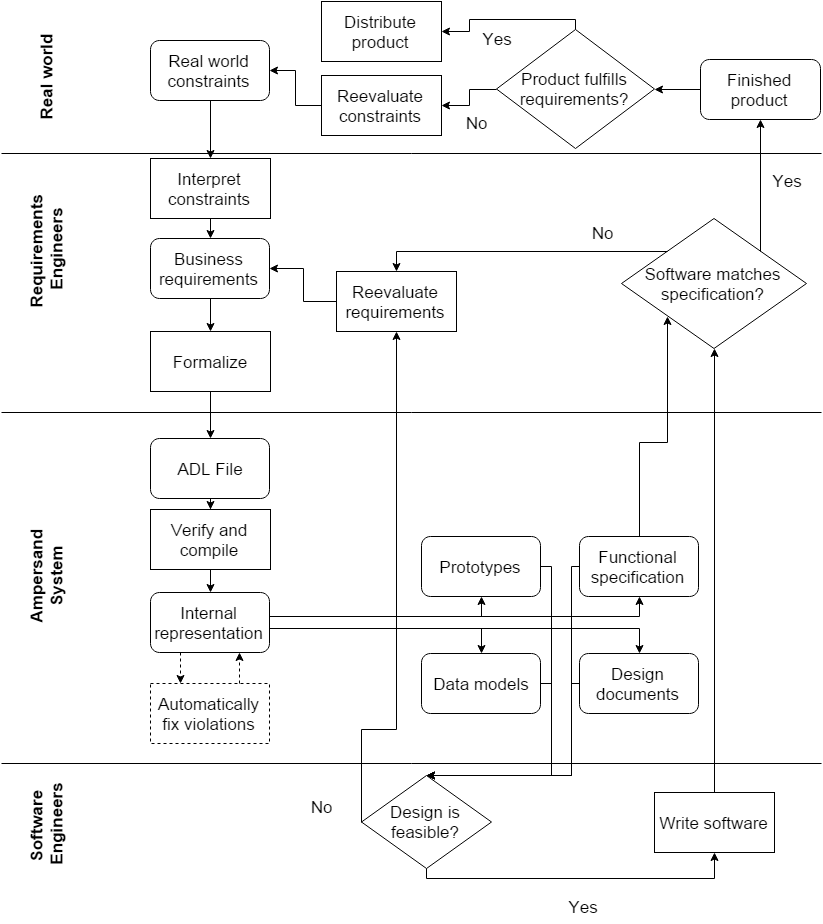
\includegraphics[width=0.6\textwidth]{../figures/business_process}
\caption{The role of Ampersand in the software design cycle}~\label{fig:BusinessProcess}
\end{center}
\end{figure}

Figure \ref{fig:BusinessProcess} is a simplified view of the software design
cycle, intended to highlight the role of Ampersand in this cycle. This view
omits many of the uses of the design artifcats generated by Ampersand; instead
it focuses mainly on the primary purpose, which is to help create a finished
software system. The contribution of this project is denoted with dashed lines.

\section{Business Data Model and Data Dictionary}\label{sec:DataModel}

\section{The Scope of the Product}\label{sec:ScopeOfProduct}
\section{Functional Requirements}\label{sec:Functional}
\subsection{Input}
\subsection{Correct Translation of Input}
\subsection{Output}

\chapter{Non-functional Requirements}\label{ch:NonFunc}
\section{Look and Feel Requirements}\label{sec:LookAndFeel} 
\section{Usability and Humanity Requirements}\label{sec:Usability}
\section{Performance Requirements}\label{sec:Performance}
\section{Operational and Environmental Requirements}\label{sec:Operational}
\section{Maintainability and Support Requirements}\label{sec:Support}
\section{Security Requirements}\label{sec:Security}
\section{Cultural Requirements}\label{sec:Cultural}
\section{Legal Requirements}\label{sec:Legal}
The implementation must eventually be included in Ampersand, which is licensed
under GPL3. To comply with this license, all of the implementation code must be
either written by us so we may license it under GPL, or must already be licensed
under GPL, or a compatible license, by its original author. We do not plan to
use existing code, other than as a reference.
\edcomm{YS}{Rephrase this one, I wanted to put forward the idea}%
\edcomm{YT}{I rephrased it more concretely: we have to follow the license agreement of
Ampersand, which appears to be GPL3. That means all the code we include must
either be our own so we can place it under that license, or must already be
under GPL. I don't see any reason we couldn't take code from somewhere if it was
GPL. }%
\chapter{Project Issues}\label{ch:issues}
\section{Open Issues}\label{sec:issues}
\section{Off-the-Shelf Solutions}\label{sec:solutions}
\section{New Problems}\label{sec:NewProblems}
\section{Tasks}\label{sec:Tasks}
\section{Migration to the New Product}\label{sec:Migration}
Upon final review by the client and intensive testing, if the client is
satisfied by the quality of code and its maintainability, the implementation
will be made part of the production stream.  This process is quite simple due to
the nature of the project; the core development team of Ampersand is quite
small, and the project is hosted on GitHub; so our migration will consist of
submitting a pull request to the Ampersand repository.
\section{Risks}\label{sec:Risks}
\begin{itemize}
\item The new code must not introduce any 
errors or performance regressions
into Ampersand.
\item The code must satisfy existing tests and 
additional tests written for the new algorithm being implemented.
\end{itemize}

\section{Costs}\label{sec:Costs}
Currently the software is open source maintained by Tarski Systems.
All the software used in Ampersand are also open source
There will no change in cost as a result of our implementation. The client ( Tarski Systems)
will be responsible for managing the cost of maintenance of the software in the future.
\section{User Documentation and Training}\label{sec:UserDoc}
\section{Waiting Room}\label{sec:Waiting}
\section{Ideas for Solutions}\label{sec:Solutions}


\bibliographystyle{alpha}
\bibliography{SRS}
\end{document}










